\documentclass{standalone}
\usepackage{tikz}
\usetikzlibrary{calc}

\begin{document}
\begin{tikzpicture}[scale=1.5]

% Define the function
\newcommand{\f}[1]{3*#1^2}

% Draw the axes
\draw[->] (-2,0) -- (4,0) node[right] {$x$};
\draw[->] (0,-2) -- (0,8) node[above] {$y$};

% Plot the curve
\draw[blue, thick] plot[domain=-2:4] (\x, {\f{\x}});

% Calculate the point where the tangent line touches the curve at x=2
\pgfmathsetmacro{\tanPointX}{2}
\pgfmathsetmacro{\tanPointY}{\f{\tanPointX}}

% Draw the tangent line at x=2
\draw[red, thick] (\tanPointX,-2) -- (\tanPointX,8);

% Fill the region between the curve and the tangent line from x=0 to x=2
\fill[green!30] plot[domain=0:\tanPointX] (\x, {\f{\x}}) -- (\x,0) -- cycle;

% Mark the intersection point in green
\fill[green, circle, inner sep=1pt] (\tanPointX,\tanPointY) node[below right] {Green Intersection};

% Label the tangent line
\node[red, below left] at (2,-0.5) {Tangent Line};

\end{tikzpicture}
\end{document}